\PassOptionsToPackage{unicode}{hyperref}
\documentclass[aspectratio=43, professionalfonts, 9pt]{beamer}

\usefonttheme[onlymath]{serif}
\usetheme[showtotalframes]{tudo}

\ifluatex
  \usepackage{polyglossia}
  \setmainlanguage{german}
\else
  \ifxetex
    \usepackage{polyglossia}
    \setmainlanguage{german}
  \else
    \usepackage[german]{babel}
  \fi
\fi


% Mathematik
\usepackage{amsmath}
\usepackage{amssymb}
\usepackage{mathtools}
\usepackage{braket} %von mir
\usepackage{cancel}

\usepackage{hyperref}
\usepackage{bookmark}
\usepackage{booktabs}  %von mir
\usepackage{animate}
\usepackage{graphicx} %von mir
\usepackage[autostyle]{csquotes}

\iffalse
\newcommand{\bunderbrace}[2]{
  \begin{array}[t]{@{}c@{}}
  \underbrace{#1}\\
  #2
  \end{array}
  \fi
}

%%%%%%%%%%%%%%%%%%%%%%%%%%%%%%%%%%%%%%%%%%%%%%%%%%%%%%%%%%%%%%%%%%%%%%%%%%%%%%%%
%%%%%-------------Hier Titel/Autor/Grafik/Lehrstuhl eintragen--------------%%%%%
%%%%%%%%%%%%%%%%%%%%%%%%%%%%%%%%%%%%%%%%%%%%%%%%%%%%%%%%%%%%%%%%%%%%%%%%%%%%%%%%

%Titel:
\title{Analyse von Polymerkonfigurationen mit Neuronalen Netzen}
%Autor
\author[C.~Vorsmann]{Clemens Vorsmann}
%Lehrstuhl/Fakultät
\institute[Theoretische Physik I]{AG Kierfeld \\  Fakultät Physik}
%Titelgrafik
%\titlegraphic{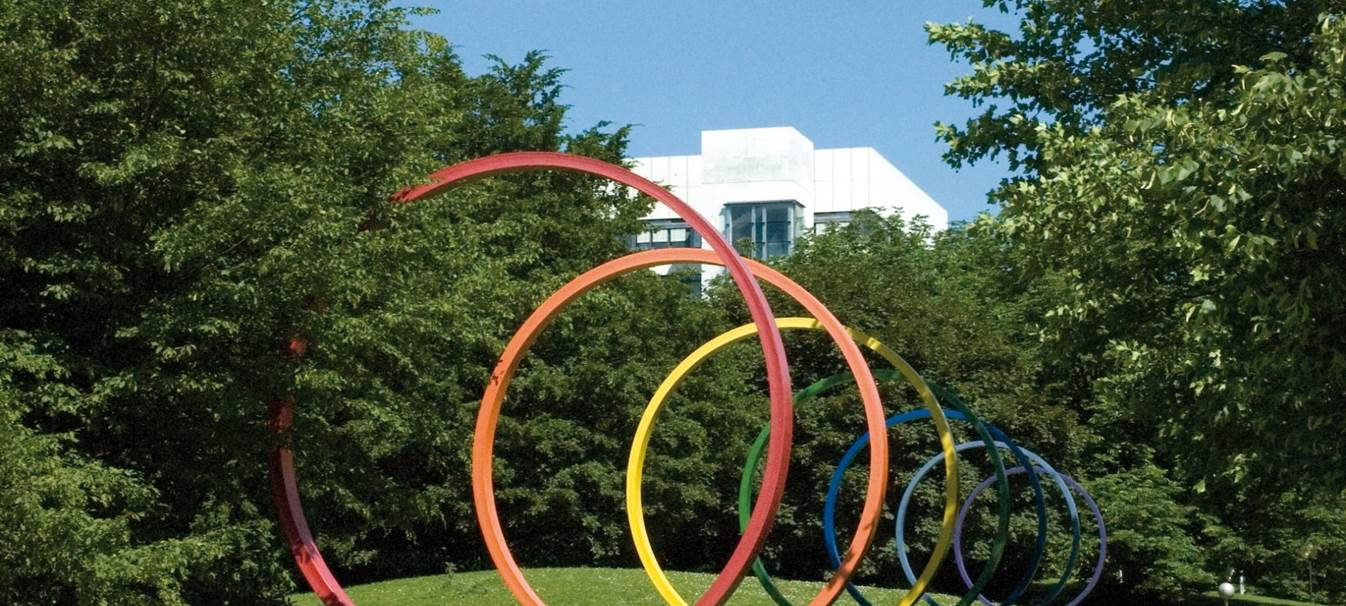
\includegraphics[width=0.7\textwidth]{images/tudo-title-2.jpg}}


\begin{document}

\maketitle

%\section{Einleitung}

\begin{frame}
\frametitle{Inhaltsübersicht}
\tableofcontents%[pausesections]
\end{frame}


\section{Einleitung}
\begin{frame}
  \frametitle{Worum gehts?} %die mesten horen wahrscheinlch floquet theorie zum ersten mal, deshalb nochmal etwas genauer, worum es geht
  \textbf{Motivation}
    \begin{itemize}
      \item Nur wenige quantenmechanische Systeme exakt analytisch l"osbar
      \item Zeitabh"angige Systeme meistens nur im Rahmen der St"orungstheorie betrachtbar

      $\rightarrow$ Beschr"anken auf Probleme, die periodisch in der Zeit sind
    \end{itemize}

  \textbf{Floquet-Theorie}
  \begin{itemize}
    \item 1883 von Gaston Floquet
    \item mathematische Theorie von linearen gew"ohnlichen DGL's der Form $\dot f(t)=A(t)f(t)$ mit $A(t)=A(t+T)$
  \end{itemize}




\end{frame}
%im rahmen der floquet thoery kann man solche dgls dann l;sen  indem man die eigenwertgleichung fuer den neuen zeitabh op loest
%in meiner arbeit hab ich das konkret aber nicht gebraucht. den einzelnen sowie die gekoppelten oszis konnte man mit anderen tricks loesen. mit der lsg konnte ich dan aber das floquet theorem bestaetigen, indem eben die quasie energien und floquet moden identifiziert werden.
%anwendung der reulstate der floquet theorie hatte man aber bei den berechnungen der erwartungswerte der energie, wie sich zeigen wird

\section{Grundlagen der Floquet-Theorie}
%im rahmen der quantenmechanikn hier noch fur bel Hamiltonop
\begin{frame}
  \textbf{Floquet-Theorem} %kern der ganzen sache
  \begin{itemize}
    \item Schr"odinger-Gleichung mit periodischem Hamilton-Operator $H(t)=H(t+T)$
    \begin{equation}
      \text i\hbar \frac{\partial}{\partial t} \Psi_n(x,t) = H(t)\Psi_n(x,t)
    \end{equation}

    $\rightarrow$ L"osungen haben die Form
    \begin{equation}
      \Psi_n(x,t)=\exp\left(-\frac{\text i}{\hbar}\epsilon_nt\right)\Phi_n(x,t)
    \end{equation}

    \item Floquet-Moden $\Phi_n(x,t)=\Phi_n(x,t+T)$ und Quasienergien $\epsilon_n$
  \end{itemize}
  %bloch theorem der zeit

  \textbf{Eigenwertproblem}
  \begin{equation} %einsetzen des ansatzes in s glg
    \epsilon_n \Phi_n(x,t) = \left(H(t)-\text i\hbar \partial t\right) \Phi_n(x,t)
  \end{equation}
  %bei oszis nicht gebraucht

  \textbf{Mittlerer Erwartungswert der Energie } %zustand psi n
  \begin{equation}%gemittelten erwartungswert berechenbar, ohne den eigentlichen zeitabhaengigen zu kennen, nur von den quasienergien abhaengig
    \bar H_n = \epsilon_n-\omega \frac{\partial}{\partial \omega} \epsilon_n
  \end{equation}
  \begin{itemize}
   \item $\omega=2\pi/T$
 \end{itemize}
\end{frame}






\section{Periodisch getriebener harmonischer Oszillator}
\subsection{L"osung}
\begin{frame}
  \textbf{Hamilton-Operator}
  \begin{equation} %treibende kraft S beliebieg aber periodisch
    H(t) = H(t+T) = \frac{p^2}{2m} + \frac{1}{2}m\omega_0^2x^2-S(t)x
  \end{equation}
  \textbf{L"osung der Schr"odinger-Gleichung}
  \begin{enumerate}
    \item Variablenwechsel $x \rightarrow y=x-\zeta(t)$ %so wie bei oszi in auserem e feld nur mit zeitabhaengiger verschiebeung
    %impulsoperator aendert sich nicht, mit kettenregel ableitung bleibt identisch
    \item Unit"are Transformation $\Psi(y,t) = \exp\left(\frac{\text i}{\hbar}m\dot \zeta(t) y\right)\Lambda(y,t)$
    \begin{itemize}
      \item $L(\zeta(t),\dot \zeta(t), t) = \frac{1}{2}m\dot \zeta(t)^2 - \frac{1}{2}m\omega_0^2\zeta(t)^2 + S(t)\zeta(t)$
      \item   $m\ddot \zeta(t) + m\omega_0^2\zeta(t) - S(t) = 0$

      $\rightarrow$ $\zeta(t)$ schwingt klassisch
      %durch umstellen lagrangefunkt und klass bewegungsgleichung des getriebene oszis fuer verschiebung zeta identifiziert
    \end{itemize}
    \item Unit"are Transformation  $\Lambda(y,t) = \exp\left(\frac{\text i}{\hbar}\int_0^tL(\zeta(t'),\dot \zeta(t'), t') \: \text d t'\right)\chi(y,t)$

    $\rightarrow$ ungetriebener Oszillator $\chi(y,t)$
  \end{enumerate}
  %hier ergibt sich dann fuer chi die stat schroed gleichung des standart oszillators, dessen lsgen wir ja kenne, also ist mit den drei transformationen die lsg fur den getriebenen oszi bekannt, die sind dan wegen chi auch auf r normiert, wenn man dan dort egen die richtige norm konstante nimmt
\end{frame}

\begin{frame}
  \textbf{Wellenfunktionen}
  \begin{align}
    &\Psi_n(x,t) = N_nH_n\left(\sqrt{\frac{m\omega_0}{\hbar}}(x-\zeta(t))\right) \exp\left[\frac{-m\omega_0}{2\hbar}(x-\zeta(t))^2\right] \notag\\
    & \cdot \exp\left[\frac{\text i}{\hbar}\left(m\dot \zeta(t)(x-\zeta(t))-E_nt+\int_0^tL(\dot \zeta(t'),\zeta(t'),t')\:\text dt'\right)\right] \; ,
    \; n \in \mathbb{N}_0
    %um klassische lsg verschobene ungetriebene lsg mit extra phase
    %treibende kraft geht stets ueber klass lsg und direkt ueber die die lagrangefunktion ein
  \end{align}
  \begin{itemize}
    \item $N_n = \left(\frac{m\omega_0}{\pi \hbar}\right) \frac{1}{\sqrt{2^nn!}}$,
     $E_n = \hbar \omega_0(n+1/2)$ %eignenergien des ungetr oszis
  \end{itemize}

  \textbf{Floquet-Theorem}
  %bisl umstellen um Floquet theorem zu bestaetigen
  \begin{itemize}
    \item Quasienergien $\epsilon_n = E_n - \frac{1}{T} \int_0^T L(\dot \zeta(t), \zeta(t), t) \: \text d t$
    %alles lineare im exponenten, lagrangefunktion periodisch oder konstanter term, der nach integrieren linear in t ist
    \item Floquet-Moden
    \begin{align}
        &\Phi_n(x,t) =
         N_nH_n\left(\sqrt{\frac{m\omega_0}{\hbar}}(x-\zeta(t))\right) \exp\left[\frac{-m\omega_0}{2\hbar}(x-\zeta(t))^2\right] \notag\\
        & \cdot \exp\left[\frac{\text i}{\hbar}\left(m\dot \zeta(t)(x-\zeta(t))+\int_0^tL(\dot \zeta(t'),\zeta(t'),t')\:\text d t'-\frac{t}{T} \int_0^T L(\dot \zeta(t),\zeta(t),t)\:\text dt\: \right)\right] \; ,\notag\\
        & n \in \mathbb{N}_0
    \end{align}
  \end{itemize}
\end{frame}


\subsection{Quasienergien}
\begin{frame}
  \frametitle{Quasienergien f"ur sinusf"ormige Treibkraft}
  \textbf{Treibkraft}
  \begin{equation}
    S(t)=A\sin(\omega t)
  \end{equation}

  \textbf{Klassische L"osung}
  %EINE lsg, allgmeine homogene lsg=0 (nur noch die spezielle), um es einfach zu machen. wie die lsg tats"achlich aussieht, haengt natuerlich von anfangsbedingungen ab
  \begin{equation}
    \zeta(t) = \frac{A\sin(\omega t)}{m(\omega_0^2 - \omega^2)} \;
  \end{equation}

  \textbf{Quasienergien}
  \begin{equation}
    \epsilon_n  = E_n - \frac{A}{4m(\omega_0^2-\omega^2)} \;.
  \end{equation}
  %durch treibkraft konstant verschoben, mittelwert h divergiert wenn treibfrequenz omega nahe an oszieigenfrequenz omega_0
\end{frame}

\begin{frame}
  \frametitle{Quasienergien f"ur beliebige Treibkraft}
  \textbf{Treibkraft}%bel periodische funktion, rechteck, dreieck
  %furierreihenansatz
  \begin{equation}
    S(t) = \sum_{j=-\infty}^\infty c_j \text e^{\text ij\omega t}, \; c_j = \frac{1}{T} \int_0^T S(t) \text e^{-\text ij\omega t} \: \text d t
  \end{equation}

  %gleichen ansatz fur klassische lsg, nur andere koeff, danneinsetzen in begsglg ung koefvergleich
  \textbf{Klassische L"osung}
  \begin{equation}
    \zeta(t) = \sum_{j=-\infty}^\infty d_j \text e^{\text ij\omega t}
  \end{equation}


  %lagrangefkt bilden -> doppelsummen wegen quadrat->linearer teil des integrals rauskriegen und dann wie oben bilden (das auser die E_n ist ja der lin teil)
  \textbf{Quasienergien}
  \begin{align}
    \begin{split}
      \epsilon_n &= \hbar \omega_0\left(n+\frac{1}{2}\right) - \sum_{j \in \mathbb Z} \frac{c_jc_{-j}}{2m(\omega_0^2-j^2\omega^2)}
    \end{split}
  \end{align}

\end{frame}



\subsection{Erwartungswerte}
\begin{frame}
  \frametitle{Ort}
  \textbf{Betrag der Wellenfunktion}
  \begin{equation}
    |\Psi_n(x,t)|^2=|\Psi_{n,\text{ungetrieben}}(x-\zeta(t),t)|^2
  \end{equation}

  \textbf{Erwartungswerte}
  \begin{itemize}
    \item
  \begin{align}
    \begin{split}
      \braket{x}_n &= \int_{-\infty}^{\infty} |\Psi_{n,\text{ung}}(x-\zeta(t),t)|^2 x \: \text dx
      = \int_{-\infty}^{\infty} |\Psi_{n,\text{ung}}(y,t)|^2 (y+\zeta(t)) \: \text dy \\
      &= \braket{y+ \zeta(t)}_{n,\text{ung}} = \braket{y}_{n,\text{ung}} + \zeta(t) = \zeta(t) \; .
      \label{erwartungswert_x_einzelner}
    \end{split}
  \end{align}

    \item
  \begin{equation}
    \braket{x^m}_n = \braket{(y+\zeta(t))^m}_{n,\text{ung}} = \sum_{j=0}^m \begin{pmatrix} m \\ j \\ \end{pmatrix} \braket{y^{m-j}}_{n,\text{ung}}\zeta^j(t) \;
    \label{erwartungswert_x^m_einzelner}
  \end{equation}
  \end{itemize}

\end{frame}




\begin{frame}
  \frametitle{Impuls}
  \textbf{Erwartungswerte}
  \begin{itemize}
    \item
    \begin{align}
      \braket{p}_n = \braket{p_y+ m\dot\zeta(t)}_{n,\text{ung}} = m\dot{\zeta}(t) \;
      \label{erwartungswert_p_einzelner}
    \end{align}

    \item
    \begin{equation}
        \braket{p^m}_n = \braket{(p_y+m\dot\zeta(t))^m}_{n,\text{ung}} = \sum_{j=0}^m\begin{pmatrix} m \\ j \\ \end{pmatrix} \braket{p_y^{m-j}}_{n,\text{ung}}(m\dot\zeta(t))^j \; .
        \label{erwartungswert_p^m_einzelner}
    \end{equation}
  \end{itemize}
\end{frame}


\begin{frame}
  \frametitle{Heisenberg-Unsch"arferelation}
  \begin{align}
    \Delta x_n\Delta p_n &= \sqrt{\braket{x^2}_n-\braket{x}^2_n}\sqrt{\braket{p^2}_n-\braket{p}^2_n} \notag\\
    &= \sqrt{s^2(2n+1)+\zeta^2(t)-\zeta^2(t)}\sqrt{m^2\omega^2_0s^2(2n+1)+m^2\dot\zeta^2(t)-m^2\dot\zeta^2(t)} \notag\\
    &= \frac{\hbar}{2}(2n+1) \;
  \end{align}
  \begin{itemize}
    \item  $s = \sqrt{\frac{\hbar}{2m\omega_0}}$
  \end{itemize}
\end{frame}



\begin{frame}
  \frametitle{Energie}
  \textbf{Erwartungswert}
  \begin{align}
    \braket{H}_n = E_n - L(\dot{\zeta},\zeta,t) + m\dot{\zeta}^2(t) \;
    %hier en in extra zeile mit satz definieren evt
  \end{align}

  \textbf{Zeitliches Mittel}
  \begin{itemize}
    \item Beliebige Treibkraft
    \begin{align}
      \overline{H}_n = \epsilon_n - \omega\frac{\partial}{\partial \omega}\epsilon_n
      = E_n - \sum_{j=-\infty}^{\infty} \left[ \frac{c_jc_{-j}}{2m(\omega_0^2-j^2\omega^2)}\left( 1-\frac{2j^2\omega^2}{(\omega_0^2-j^2\omega^2)}\right) \right] \; .
    \end{align}

    \item Sinusf"ormige Treibkraft
    \begin{equation}
      \overline{H}_n = E_n - \frac{A}{4m(\omega_0^2-\omega^2)}\left(1-\frac{2\omega^2}{(\omega_0^2-\omega^2)}\right) \; .
      \label{mittleres_H}
    \end{equation}
  \end{itemize}
\end{frame}





\section{Gekoppelte getriebene Oszillatoren}
\subsection{L"osung}
\begin{frame}
  \textbf{Hamilton-Operator}
  \begin{equation}
    H(t) = H(t+T) = \frac{p_1^2}{2m} + \frac{p_2^2}{2m} + \frac 1 2 kx_1^2 + \frac 1 2 kx_2^2 + \frac 1 2 \kappa(x_2-x_1)^2 - S(t)x_1 \;
    \label{H_gekoppelt}
  \end{equation}
  \begin{itemize}
    \item Kopplungsterme $\propto x_1x_2$ st"oren, kein Produktansatz m"oglich
  \end{itemize}

  \textbf{L"osung der Schr"odinger-Gleichung}
  \begin{enumerate}
    \item Koordinatentransformation entkoppelt $H(x_1,x_2,p_1,p_2,t)$ zu unabh"angigen $H_+(x_+,p_+,t)$ und $H_-(x_-,p_-,t)$
    %keine kopplungsterme x+x-
    \item Produktansatz $\Psi_{n,l}(x_+,x_-,t)=\Psi_{+,n}(x_+,t)\Psi_{-,l}(x_-,t)$
  %\end{enumerate}

    $\rightarrow$ Unabh"angige Schr"odinger-Gleichungen f"ur einzelnen (getriebenen) Oszillator
  \end{enumerate}
\end{frame}



\begin{frame}
  \frametitle{Unit"are Koordinatentransformation}
  \textbf{Neuen Koordinaten}
  \begin{equation}
    x_+ = \frac{1}{\sqrt{2}}(x_2+x_1) \;,\; x_-=\frac{1}{\sqrt{2}}(x_2-x_1) \;,
    \label{koord_trafo_x}
  \end{equation}
  \begin{itemize}
    \item Folgt aus den normierten Eigenvektoren des klassischen Problems
  \end{itemize}

  \textbf{Ortsoperatoren,Impulsoperatoren}
  \begin{itemize}
    \item $x_1=\frac{1}{\sqrt{2}}(x_+-x_-) \;,\; x_2=\frac{1}{\sqrt{2}}(x_++x_-)$ $p_1=\frac{1}{\sqrt{2}}(p_+-p_-) \;,\; p_2=\frac{1}{\sqrt{2}}(p_++p_-)$
    \item $x_1^2+x_@^2=x_+^2+x_-^2$ $p_1^2+p_2^2=p_+^2+p_-^2$
  \end{itemize}
\end{frame}

\begin{frame}
  \textbf{Hamilton-Operator}
  \begin{align}
    H(t) &= H(t+T) = \frac{p_1^2}{2m} + \frac{p_2^2}{2m} + \frac 1 2 kx_1^2 + \frac 1 2 kx_2^2 + \frac 1 2 \kappa(x_2-x_1)^2 - S(t)x_1 \notag\\
    &= \frac{p_+^2}{2m}+\frac{1}{2}kx_+^2-\frac{1}{\sqrt{2}}S(t)x_+  +
    \frac{p_-^2}{2m}+\frac{1}{2}(k+2\kappa)x_-^2+\frac{1}{\sqrt{2}}S(t)x_- \notag\\
    &= \frac{p_+^2}{2m}+\frac{1}{2}k_+x_+^2-S_+(t)x_+  +
    \frac{p_-^2}{2m}+\frac{1}{2}k_-x_-^2-S_-(t)x_- \notag\\
    &= H_+(x_+,p_+,t) + H_-(x_-,p_-,t) \;,\; H_\pm:\cal H_\pm \rightarrow \cal H_\pm \; .
    \label{gekoppelte_H_entkoppelt}
  \end{align}
  \begin{itemize}
    \item $w_+=\sqrt{\frac{k}{m}}$, $ \omega_-=\sqrt{\frac{k+2\kappa}{m}}$
  \end{itemize}
\end{frame}




\begin{frame}
  \frametitle{Produktansatz}
  \textbf{Unabh"angige Schr"odinger-Gleichungen}
  \begin{align}
    &\text i\hbar \frac{\partial}{\partial t} \Psi_{n,+}(x_+,t) = H_+(x_+,t)\Psi_{n,+}(x_+,t) \\\notag
    &\text i\hbar \frac{\partial}{\partial t} \Psi_{n,-}(x_-,t) = H_-(x_-,t)\Psi_{n,-}(x_-,t)
  \end{align}

  \textbf{Wellenfunktion}
  \begin{align}
     &\Psi_{n,l}(x_+,x_-,t) = \Psi_{+,n}(x_+,t)\Psi_{-,l}(x_-,t) \notag\\
     &=N_{n,+}H_n\left(\sqrt{\frac{m\omega_+}{\hbar}}(x_+-\zeta_+(t))\right) \exp\left(\frac{-m\omega_+}{2\hbar}(x_+-\zeta_+(t))^2\right)\notag\\
     &\quad \cdot \exp\left[\frac{\text i}{\hbar}\left(m\dot \zeta(t)(x_+-\zeta_+(t))-E_{+,n}t+\int_0^tL_+\:\text dt'\right)\right] \quad\quad\quad\notag\\
     &\quad \cdot N_{l,-}H_l\left(\sqrt{\frac{m\omega_-}{\hbar}}(x_--\zeta_-(t))\right) \exp\left(\frac{-m\omega_-}{2\hbar}(x_--\zeta_-(t))^2\right)\notag\\
     &\quad \cdot \exp\left[\frac{\text i}{\hbar}\left(m\dot \zeta(t)(x_--\zeta_-(t))-E_{-,l}t+\int_0^tL_-\:\text dt'\right)\right] \;,\; \Psi_\pm \in \cal H_\pm
   \end{align}

\end{frame}



























b

\section{Simulation}
\subsection{Polymermodell}

\begin{frame}
       \begin{tabular}{cl}
         \begin{tabular}{c}
           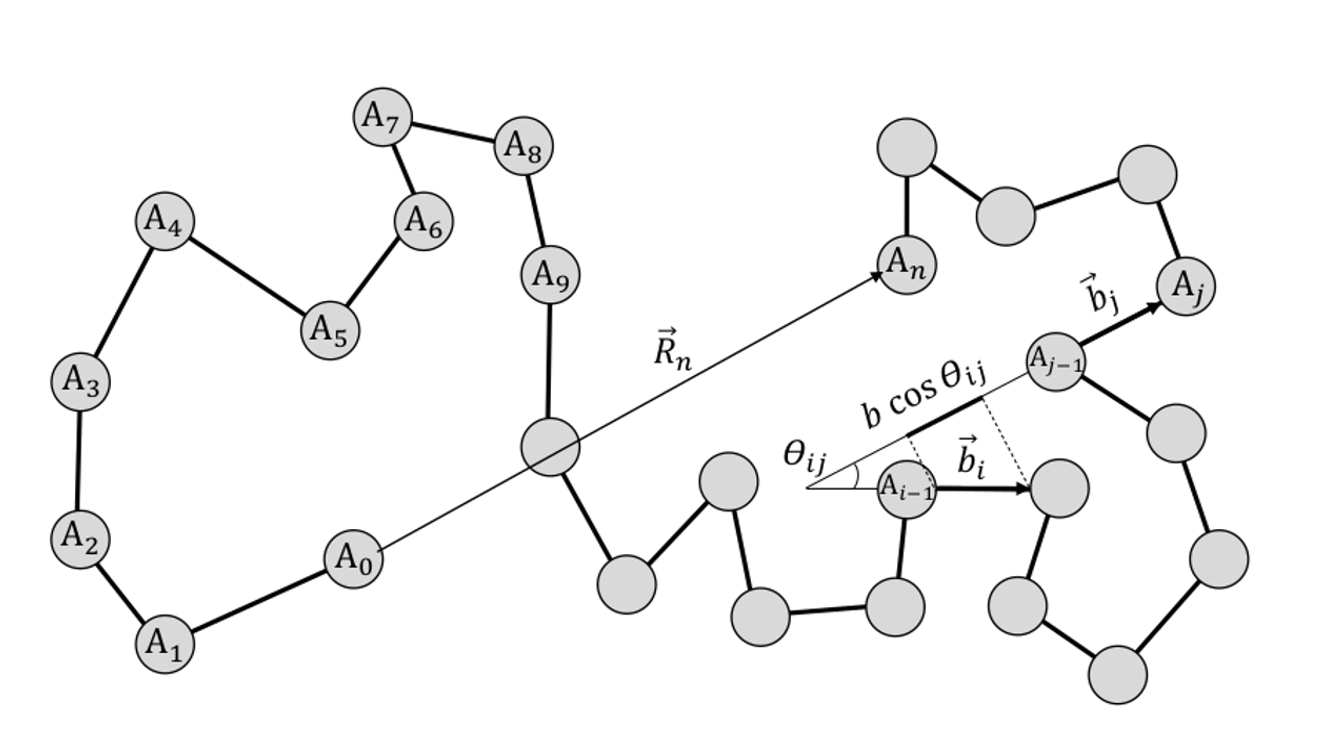
\includegraphics[width=0.5\textwidth]{Plots/rubinstein.png}
           \end{tabular}
           & \begin{tabular}{l}
             \parbox{0.5\linewidth}{
             \begin{itemize}
               \setlength\itemsep{1em}
               \item Monomere bestehen aus \textit{beads}\\ und \textit{bonds} \\
               \item N Monomere \\(Polymerisationsgrad)
               \item Bondvektoren $\vec{b}_i$ mit Länge $b$ \\
             \end{itemize}

             }
             \end{tabular}  \\
         \end{tabular}
         \begin{tiny}Quelle: Rubinstein, Michael and Colby, Ralph H. - Polymer Physics\\
         \end{tiny}
         \begin{itemize}
           \item $\Theta_{ij}$ ist Winkel zwischen $\vec{b}_i$ und $\vec{b}_j$ \\
           \item End-zu-End-Abstand $\vec{R}=\sum_{i=0}^{N-1} \vec{b}_i$
         \end{itemize}
\end{frame}

%\begin{frame}
%  \frametitle{wichtige Messgrößen}
%  \begin{block}{Definitionen}
%     \begin{itemize}
%       \item $\langle O \rangle = \frac{1}{Z} \sum_{i} O \text{e}^{-\beta E_i}$
%       \item $Z = \sum_i \text{e}^{-\beta E_i}$
%       \item $\langle R^2 \rangle = b^2 \sum_{i=0}^{N-1} \sum_{j=0}^{N-1} \langle \text{cos} \, \Theta_{ij} \rangle$
%       \item $\vec{t}_i = \frac{\vec{b}_i}{b}$
%       \item $\vec{t}_i \cdot \vec{t}_j = \text{cos} \, \Theta_{ij}  = \text{exp}{\left(- \frac{\lvert i - j \rvert}{ L_{\mathrm{p} }} \right)} $
%     \end{itemize}
%  \end{block}
%\end{frame}
\begin{frame}
   \frametitle{Wormlike-Chain (WLC)}
   \begin{block}{Definition über die Biegeenergie}
     \begin{itemize}
       \item $\vec{t}_i = \frac{\vec{b}_i}{b}$
       \item $\kappa = E \cdot I \sim E \cdot a^4$
       \item $E_{\text{bond}} = \frac{\kappa}{b} (1 - \text{cos}\,\Theta_{i-1,i})$
       \item $E_{\mathrm{Biege}}^{\mathrm{Ges}} = \frac{\kappa}{2b}\,\sum_{i=1}^{N-1} \left( \vec{t}_{i-1} - \vec{t}_{i}  \right)^2$
       \item $ \langle \vec{t}_i \cdot \vec{t}_j \rangle = \langle \text{cos} \, \Theta_{ij} \rangle  = \text{exp}{\left(- \frac{\lvert i - j \rvert}{ L_{\mathrm{p} }} \right)} $
     \end{itemize}
   \end{block}
   \begin{block}{Persistenzlänge der WLC}
     \begin{itemize}
       \item $L_{\mathrm{p}} = -\frac{b}{\coth \frac{\kappa}{b\,\mathrm{k_B\,T}} - \frac{b}{\kappa}\,\mathrm{k_B} \, T }$
     \end{itemize}
  \end{block}
\end{frame}

\begin{frame}
  \frametitle{Klassifizierung nach Flexibilität}
  \begin{figure}
    \centering
    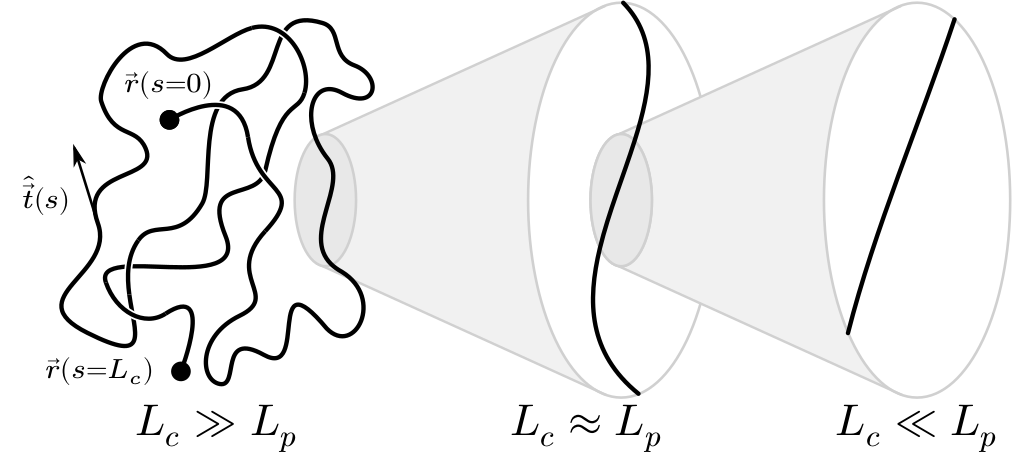
\includegraphics[width=\textwidth]{Plots/regime.png}
    \caption{Quelle: Dissertation Tobias Kampmann}
    \label{fig:regime}
  \end{figure}
\end{frame}

\subsection{Monte-Carlo Simulation}

\begin{frame}
  \frametitle{Markow-Sampling}
  \begin{itemize}
    \item Berechnung von Erwartungswerten, mittels Zufallsprozessen
    \item Sampling vereinfacht Erwartungswert zu $\langle O \rangle = \frac{1}{n} \sum_{i=0}^n O(i)$
    \item Dafür zwei Bedingungen: \\
          \begin{enumerate}
            \item Detailliertes Gleichgewicht
            \item Ergodizität
          \end{enumerate}
  \end{itemize}
  \begin{block}{Detailliertes Gleichgewicht}
    \begin{itemize}
      \item $\frac{m_{ij}}{m_{ji}} = \frac{p_j}{p_i}$
    \end{itemize}
  \end{block}
\end{frame}

\begin{frame}
  \frametitle{Metropolis Algorithmus}
  \begin{itemize}
    \item Vorschlagsmoves mit Vorschlagswahrscheinlichkeit $V_{ij}$
    und Akzeptanzwahrscheinlichkeit $A_{ij}$
    \item $m_{ij} = V_{ij}A_{ij}$
  \end{itemize}
  \begin{block}{Metropolis-Filter}
    \begin{itemize}
      \item $A_{ij} = \text{min}( 1, \frac{p_i}{p_j})$
      \item $V_{ij} = V_{ji}$
    \end{itemize}
  \end{block}
  \begin{itemize}
    \item $p_i \propto \text{exp}(-\beta E_i)$
  \end{itemize}
\end{frame}

\begin{frame}
  \frametitle{Monte-Carlo-Moves}
  \begin{enumerate}
    \item Wähle zufälligen Bead
    \item Drehe zugehörigen Bondvektor, um $\Delta\Theta$
    \item $\Delta E = E_{\text{alt}}-E_{\text{neu}}$
    \item Fallunterscheidung:\\
         \setbeamertemplate{enumerate items}[square]
         \begin{enumerate}
           \item $\Delta E \geq 0$: akzeptiere Vorschlag
           \item $\Delta E < 0$: akzeptiere mit Wahrscheinlichkeit
                 $\text{exp}(\beta \Delta E)$
         \end{enumerate}
  \end{enumerate}
\end{frame}

\begin{frame}
\begin{minipage}[t]{0.5\textwidth}
\includegraphics[width=\textwidth]{Plots/Energie.pdf}
\end{minipage}%
\hfill%
\begin{minipage}{0.5\textwidth}
\begin{itemize}
  \item Parameter $N=100$, $b=1$, $\kappa=100$, $\beta = 1$
  \item zufällige Anfangskonfiguration
  \item Äquilibrierungszeit von ca. $10^3$ Durchläufen
  \item Äquipartitionstheorem: $\langle E \rangle = 1\,\text{k}_{\text{B}}T$
        pro Bond
\end{itemize} \vspace{2.5cm}
\end{minipage}

\end{frame}


\begin{frame}
  \frametitle{Tangentenkorrelationen}
  \begin{itemize}
    \item $L_{\mathrm{p}} = -\frac{b}{\coth \frac{\kappa}{b\,\mathrm{k_B\,T}} - \frac{b}{\kappa}\,\mathrm{k_B} \, T } \approx 99.5 $ \\
    \item $\langle \vec{t}_i \cdot \vec{t}_{i+j} \rangle = \sum_{i=0}^{N-1-j} \vec{t}_i \cdot \vec{t}_{i+j}$
  \end{itemize}
  \begin{figure}
    \centering
    \includegraphics[width=0.6\textwidth]{Plots/korr13.pdf}
    \label{fig:tangkorr}
  \end{figure}
\end{frame}

\begin{frame}
  \frametitle{Erzeugung von Messwerten}
  \begin{minipage}{0.4\textwidth}
  \begin{itemize}
    \item künstliches Neuronales Netz soll aus Polymerkonfiguration
          dessen Biegesteifigkeit bestimmen
    \item $N=100$, $b=1$, $\beta = 1$
    \item $10 \leq \kappa \leq 20$
    \item Momentaufnahme: Winkel $\Theta_{i-1,i}$, $\kappa$
  \end{itemize}
  \end{minipage}%
  \hfill%
  \begin{minipage}{0.4\textwidth}
  \includegraphics[width=\textwidth]{Plots/polymer1.pdf}
  \end{minipage}\\
  \begin{minipage}{0.4\textwidth}
    \begin{figure}
     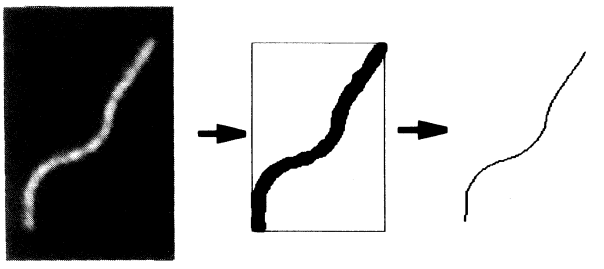
\includegraphics[width=\textwidth]{Plots/pixel-reduction.png}
     \caption{\url{https://link.aps.org/doi/10.1103/PhysRevE.48.R1642}}
    \end{figure}
  \end{minipage}%
  \hfill%
  \begin{minipage}{0.4\textwidth}
    \begin{figure}
    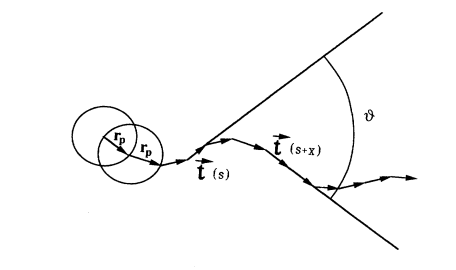
\includegraphics[width=\textwidth]{Plots/fluorescene-winkel.png}
    \end{figure}
  \end{minipage}
\end{frame}

\begin{frame}
  \frametitle{Beispielkonfigurationen}
  \begin{figure}
    \centering
    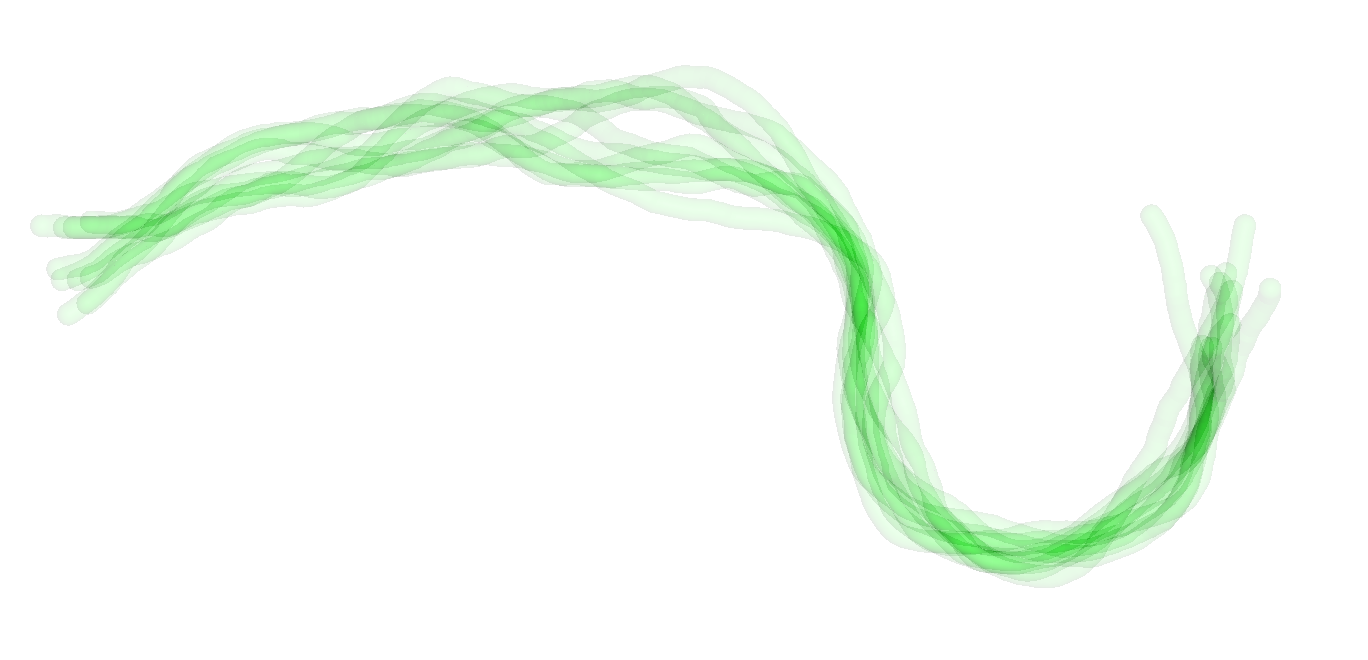
\includegraphics[width=\textwidth]{Plots/blurred33.png}
    \label{fig:bsp}
  \end{figure}
\end{frame}

\section{künstliche Neuronale Netze}
\subsection{Multilayer Perceptron}

\begin{frame}
  \frametitle{Grundlagen}
  \begin{minipage}{0.5\textwidth}
   \begin{itemize}
     \item Eingabevektor $\vec{x}_l$
     \item Gewichtmatrix $\mathbf{W}^{\left( l \right)}$
     \item Aktivierungsfunktion $g^{\left( l \right)}$
     \item maAusgabevektor $\vec{y}^{(l)}$
   \end{itemize}
  \end{minipage}%
  \hfill%
  \begin{minipage}{0.5\textwidth}
    \begin{figure}
      \centering
      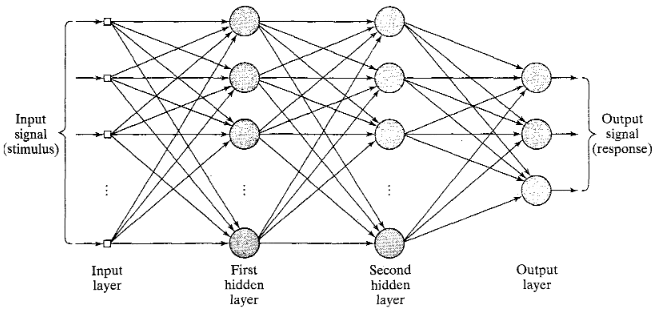
\includegraphics[width=\textwidth]{Plots/neuralnetworkhaykin.png}
      \caption{Quelle: Haykin, S.S., Neural Networks: A Comprehensive Foundation}
    \end{figure}
  \end{minipage}
\end{frame}

\begin{frame}
  \frametitle{mathematische Formulierung}
  \begin{block}{Definitionen}
    \begin{itemize}
      \item $\vec{y}^{\left( l \right)} = g^{\left( l \right)}
              \left( \bunderbrace{ \mathbf{W}^{\left( l \right)}
              \vec{x}^{\left( l \right)} + \vec{b}^{\left( l \right)}}
              {\coloneqq \vec{v}^{\left(l\right)} }  \right)$
      \item $g^{(l)}(\vec{x}^{(l)}) = g(\vec{x}^{(l)}) = ReLU \left( x \right) = \max \left ( 0,x \right)$
    \end{itemize}
  \end{block}
\end{frame}


\begin{frame}
  \frametitle{verschiedene Aktivierungsfunktionen}
  \begin{figure}
    \centering
    \includegraphics[width=0.8\textwidth]{Plots/Aktivierungsfunktionen.pdf}
  \end{figure}
\end{frame}

\subsection{Lernen und Fehlerrückführung}
\begin{frame}
  \frametitle{Ablauf des Lernalgorithmus}
  \begin{enumerate}
    \item Hinführung: Vorhersagewert $\vec{y}^{(l)}$, richtiger Wert $\vec{d}^{(l)}$
    \item Mean-squared-error (MSE) $\epsilon(n)$
    \item Fehlerrückführung: $\Delta w_{ij}^{\left( l \right)}\left(n\right)$
  \end{enumerate}
   \begin{block}{MSE, Gradientenabstiegsverfahren}
      \begin{itemize}
        \item $\epsilon \left ( n \right) = \frac{1}{2} \left( \vec{d}^{\left( l \right)}\left( n \right) -  \vec{y}^{\left( l \right)}\left( n \right)\right)^2$
        \item $\Delta w_{ij}^{\left( l \right)}\left(n\right) = - \eta \, \frac{\partial \epsilon\left(n\right)}{\partial w_{ij}^{\left( l \right)}\left(n\right) }$
      \end{itemize}
   \end{block}
\end{frame}

\begin{frame}
   \frametitle{Anpassung des Gradientenabstiegsverfahrens}
   \begin{itemize}
     \item kleine Lernrate: langsame Konvergenz
     \item große Lernrate: \enquote{Zig-Zagging}
     \item Impulskonstante $\alpha$
   \end{itemize}
   \begin{block}{Gradientenabstiegsverfahren mit Impulsterm}
      \begin{itemize}
        \item $\Delta w_{ij}^{\left( l \right)}\left(n\right) = - \eta \, \frac{\partial \epsilon\left(n\right)}{\partial w_{ij}^{\left( l \right)}\left(n\right) } + \alpha \Delta w_{ij}^{\left( l \right)}\left(n-1\right) $
      \end{itemize}
   \end{block}
\end{frame}

\begin{frame}
  \frametitle{Lern-Modi}
  \begin{itemize}
    \item Stochastic-Mode
    \item Batch-Mode
    \item Mini-Batch-Mode
  \end{itemize}
  \begin{block}{Gewichtsanpassung im Mini-Batch-Mode}
    \begin{itemize}
      \item $\Delta w_{ij}^{\left( l \right)}\left(n + 1\right) = \alpha \, w_{ij}^{\left( l \right)}\left(n + 1\right)
         + \eta \, \delta_j^{\left( l \right)}\left(n \right) \, y_i^{\left( l-1 \right)}\left(n \right)$
      \item $\delta_{j}^{\left( l \right)}\left(n \right) =
            \begin{dcases*}
              \left( d_j \left( n \right) - y_j^{\left( L \right)} \left(n \right) \right) \, g'\left( v_j^{\left(L \right)}\right)
              ,& \small{$j$-tes Perzeptron in Ausgabeschicht $L$}\\
              g'\left( v_j^{\left(l \right)}\right) \sum_{k} \delta_k^{\left(l+1\right)}\left(n\right) w_{kj}^{\left(l+1\right)}\left(n\right)
              ,& \small{$j$-tes Neuron in versteckter Schicht $l$}
            \end{dcases*}$
    \end{itemize}
  \end{block}

\end{frame}


\subsection{Trainieren des Neuronalen Netzes}

\begin{frame}
  \frametitle{Aufbau eines einfachen Modells}
  \begin{minipage}{0.5\textwidth}
    \begin{figure}
      \centering
      \includegraphics[width=\textwidth]{Plots/model_plot.pdf}
    \end{figure}
  \end{minipage}%
  \hfill%
  \begin{minipage}{0.5\textwidth}
    \begin{enumerate}
      \item input layer - 99 Neuronen
      \item hidden layer - 20 Neuronen
      \item hidden layer - 10 Neuronen
      \item output layer - 1 Neuron
    \end{enumerate}
  \end{minipage}
\end{frame}

\begin{frame}
  \frametitle{Overfitting und Early Stopping}
  \begin{figure}
    \centering
    \includegraphics[width=0.8\textwidth]{Plots/MSE.pdf}
  \end{figure}
\end{frame}

\begin{frame}
  \frametitle{Early Stopping - aber wann?}
  \begin{figure}
    \centering
    \includegraphics[width=0.8\textwidth]{Plots/MSE150k.pdf}
  \end{figure}
\end{frame}

\begin{frame}
  \frametitle{Graphische Veranschaulichung zur Validierung}
  \begin{figure}
    \centering
    \includegraphics[width=0.8\textwidth]{Plots/mlp_test_new.pdf}
  \end{figure}
\end{frame}

\begin{frame}
  \frametitle{Hyperparameteroptimierung im Vergleich}
  \begin{minipage}{0.5\textwidth}
    \begin{figure}
      \centering
      \includegraphics[width=\textwidth]{Plots/MSEOpt.pdf}
    \end{figure}
  \end{minipage}%
  \hfill%
  \begin{minipage}{0.5\textwidth}
      \begin{itemize}
        \item Konfigurationsraum \\
        \begin{enumerate}
          \item Anzahl Neuronen in den versteckten Schichten
          \item Dropoutlayer zwischen den versteckten Schichten
        \end{enumerate}
        \item Tree-Structured Parzen Estimator (TPE), jeweils 1000 Epochen
      \end{itemize}
  \end{minipage}
  \begin{minipage}{\textwidth}
     \begin{enumerate}
       \item input layer - 99 Neuronen
       \item hidden layer - 20 Neuronen
       \item dropout layer - 33.8 \%
       \item hidden layer - 8 Neuronen
       \item output layer - 1 Neuron
     \end{enumerate}
  \end{minipage}

\end{frame}

\begin{frame}
  \frametitle{Einfluss mehrerer Aufnahmen}
  \begin{minipage}{0.7\textwidth}
    \begin{figure}
      \centering
      \includegraphics[width=\textwidth]{Plots/multiple.pdf}
    \end{figure}
  \end{minipage}%
  \hfill%
  \begin{minipage}{0.3\textwidth}
    \begin{figure}
      \centering
      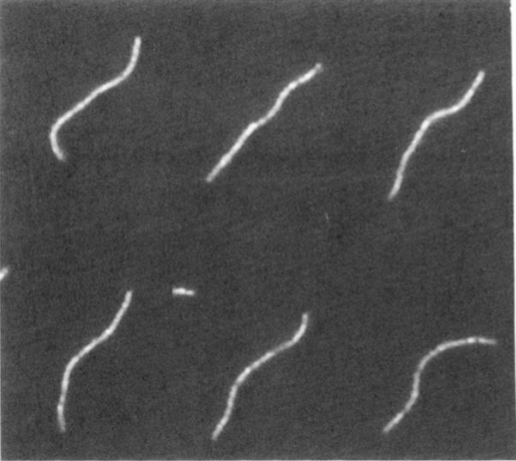
\includegraphics[width=\textwidth]{Plots/f-aktin.png}
      \caption{Quelle: \url{https://link.aps.org/doi/10.1103/PhysRevE.48.R1642}}
    \end{figure}
  \end{minipage}
\end{frame}

%\begin{frame}
%       \begin{tabular}{cl}
%         \begin{tabular}{c}
%           \includegraphics[width=0.5\textwidth]{Plots/Aktivierungsfunktionen.pdf}
%           \end{tabular}
%           & \begin{tabular}{l}
%             \parbox{0.5\linewidth}{%  change the parbox width as appropiate
%             $\text{ReLU}(x) = \text{max}(0,x)$
%                                    }
%             \end{tabular}  \\
%         \end{tabular}
%\end{frame}

\section{Fazit und Ausblick}

\begin{frame}
  \frametitle{Ausblick}
  \begin{itemize}
    \item Monte-Carlo Daten stimmen mit Theorie überein
    \item Multilayer-Perceptron eignet sich, um aus Winkelverteilung
    die Biegesteifigkeit zu bestimmen
    \item Hyperparameteroptimierung aufwendig, hier nicht erfolgreich
    \item Spare Bildverarbeitungsschritt mit Convolutional Neural Network
    \item Problem: Bild ist lediglich 2d-Projektion
  \end{itemize}
\end{frame}



\end{document}
